\documentclass[a4paper,11pt]{article}
\usepackage{tabularx}
\usepackage{graphicx}
\usepackage{wrapfig}
\usepackage{subfigure}
\usepackage{enumerate}
\usepackage{natbib}
\usepackage[center,small]{caption}
\usepackage[top=2cm, bottom=2cm, left=2.5cm, right=2.5cm]{geometry} 

\title{\huge \textbf{Tutorial on using the \textit{spartan} package to analyse agent-based simulation results}\\
\author{\Large Technique 4: Parameter Sampling and Analysis through use of the \\ 
		\Large extended Fourier Amplitude Sampling Test (eFAST), using SpartanV Interface}
\date{}
}
\begin{document}

\maketitle

\section{Introduction}
\noindent \textit{spartan}, or (\textbf{S}imulation \textbf{P}arameter \textbf{A}nalysis \textbf{R} \textbf{T}oolkit \textbf{A}pplicatio\textbf{N}) is an R package which aids the understanding of the effect aleatory and epistemic uncertainty have on the output from a simulation. This set of tutorials makes use of available example simulation output to demonstrate how a variety of methods can be applied to further understand the results that have been generated.  Following through each example should make it easier to apply the tookit to results generated by any agent-based computer simulation.  This tutorial focuses on the partitioning of variance in simulation results between input parameters, and uses a java based interface to \textit{spartan} (SpartanV) to perform this analysis.

\section{The \textit{spartan} Package}
\noindent Computer simulations are becoming a popular technique to use in attempts to further our understanding of complex systems. This package provides code for four techniques described in available literature which aid the analysis of simulation results, at both single and multiple timepoints in the simulation run. The first technique addresses aleatory uncertainty in the system caused through inherent stochasticity, and determines the number of replicate runs necessary to generate a representative result. The second examines how robust a simulation is to parameter perturbation, through the use of a one-at-a-time parameter analysis technique. Thirdly, a latin hypercube based sensitivity analysis technique is included which can elucidate non-linear effects between parameters and indicate implications of epistemic uncertainty with reference to the system being modelled. Finally, a further sensitivity analysis technique, the extended Fourier Amplitude Sampling Test (eFAST) has been included to partition the variance in simulation results between input parameters, to determine the parameters which have a significant effect on simulation behaviour.

\section{The Case Study}
\noindent The example simulation results have been taken from an ongoing project which seeks to understand the formation of lymphoid tissue in the small intestine. This simulation outputs cell behaviour measures at various points in the simulation and measures describing the development of the tissue, which occurs through interactions between the cells. Techniques 2-4 of this package allow us to explore how input parameter value affects the behaviour of these cells. We need Technique 1 to tell us how many simulation runs we need for each condition explored to ensure we have a robust representative result.

\section{Scope}
\noindent Do note that the idea of this tutorial is to demonstrate the application of the toolkit, and is not intended to act as a full introduction to using Sensitivity Analysis techniques in the analysis of simulation results. Where useful, links to further reading have been included.

\section{Prerequisites}
\begin{itemize}
\item The R statistical environment, version 2.13.1 or later.
\item The spartan R package, downloaded from the Comprehensive R Archive Network (CRAN) or from the project website.
\item The lhs and gplots R packages, available for download from CRAN.
\item The example simulation data for this tutorial, available from the project website.
\item From version 1.2 of \textit{spartan}, simulation results can be in either CSV or XML format. For earlier versions, results must be pre-processed to be in CSV format.
\item The SpartanV Java Interface for the \textit{spartan} package. Please make sure you follow the installation instructions fully prior to running this tutorial.
\item The Parameter\_Details.csv file available for download from the spartan website.
\end{itemize}

\section{Running Technique 4: eFAST Sampling and Analysis}

\noindent This technique analyses simulation results generated through parametering using the eFAST approach (extended Fourier Amplitude Sampling Test, Saltelli et al, reference below). This perturbs the value of all parameters at the same time, with the aim of partitioning the variance in simulation output between input parameters. Values for each parameter are chosen using fourier frequency curves through a parameters potential range of values. A selected number of values are selected from points along the curve. Though all parameters are perturbed simultaneously, the method does focus on one parameter of interest in turn, by giving this a very different sampling frequency to that assigned to the other parameters. Thus for each parameter of interest in turn, a sampling frequency is assigned to each parameter and values chosen at points along the curve. So a set of simulation parameters then exists for each parameter of interest.  As this is the case, this method can be computationally expensive, especially if a large number of samples is taken on the parameter search curve, or there are a large number of parameters. On top of this, to ensure adequate sampling each curve is also resampled with a small adjustment to the frequency, creating more parameter sets on which the simulation should be run. This attempts to limit any correlations and limit the effect of repeated parameter value sets being chosen. Thus, for a system where 8 parameters are being analysed, and 3 different sample curves used, 24 different sets of parameter value sets will be produced. Each of these 24 sets then contains the parameter values chosen from the frequency curves. This number of samples should be no lower than 65 (see the Marino paper for an explanation of how to select sample size). The explanation of this is greatly aided by an example, which is covered later in this tutorial.\\
\\
Once the sampling has been performed, a number of simulation runs should be performed for each set generated (this number that which has become apparent through analysis of aleatory uncertainty, or use of Technique 1 within the \textit{spartan} package). The eFAST algorithm then examines the simulation results for each parameter value set and, taking into account the sampling frequency used to produce those parameter values, partitions the variance in output between the input parameters.\\
\\
The \textit{spartan} package includes methods to both create parameter value samples using fourier frequency sampling, and to analyse the simulation results. This tutorial covers both methods.\\

\section{Parameter Sampling}
\noindent The package contains a method which can produce a parameter space sample for the parameters of interest. Simulations should then be run on each of the generated parameter sets.  This is done as follows:\\

\begin{enumerate}
\item Open the SpartanV Java interface to the \textit{spartan} package. Choose Option 6: "Generate Parameter Samples using eFAST Approach". Press Next.
\item Now we are going to declare the variables required by the package to produce the parameter value sets. Firstly, use the Directory Browser to select a folder where you wish your parameter value sets to be stored. Then, you need to enter details of each parameter for which you wish to create a range of value samples. You can do this in two ways:
\begin{itemize}
\item Press the "Add Parameter" button and add details on each parameter individually. These details will be name, baseline (calibrated) value, minimum value, and maximum value.
\item Press the "Add Parameter Values From File" button. This is much more useful if you have a large number of parameters. In this tutorial, press this button and find the Parameter\_Details.csv file you have downloaded from the website. Once you have selected this, the parameter details box will populate, as shown in Figure \ref{eFAST_Screen1}.
\end{itemize}

\item In box 3, you specify the number of resample curves you wish to employ in sampling you wish to take from the parameter space, with box 4 the specification of how many values to take from the parameter search curve. The selection of number of search curves and sampling points is covered well in the Marino and Saltelli references at the end of this document, and is thus outside the scope of this tutorial. In this example, we will employ 3 resample curves and take 65 values from the parameter space curve. Enter these values into boxes 3 and 4 and press Next.

\begin{figure}
\centering
    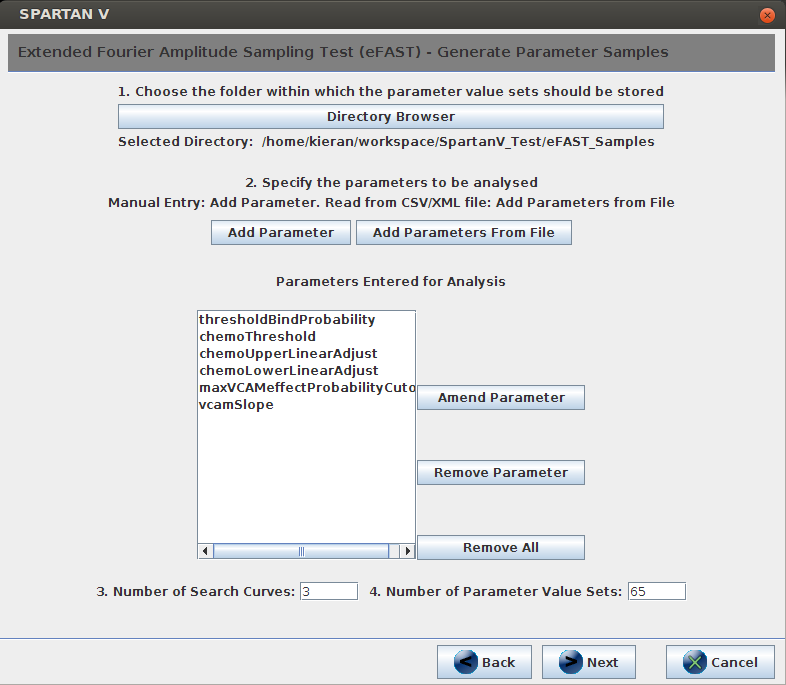
\includegraphics[width=0.8\textwidth]{SpartanV_eFAST1.png}\\ \noindent
    \caption{Specifying parameter details for eFAST parameter sampling}
    \label{eFAST_Screen1}
    \newpage 
\end{figure}

\item Press the "Generate Parameter Sample Using eFAST" button. This will produce a large number of CSV files.  Remember eFAST works by examining one parameter of interest at a time, going through the sample space using a significantly different frequency to that at which the others are sampled. Thus, for each resample curve, one set of parameter value sets is produced for each parameter of interest. Thus, in this case, we have 3 resample curves and 7 parameters (including the 'dummy'), so 24 different sets of 65 parameter samples are produced. This explains why the analysis is so computationally expensive, as this is 1560 different parameter sets on which simulations will need to be performed. Then, for each set, a number of runs are performed to produce a robust result which considers the effect of Aleatory Uncertainty (see Technique 1).  In our case, we know we need 300 runs per set of parameters to produce a robust result, meaning a total of 468,000 simulation runs.\\
\\
Each CSV file is named with the convention Curve[\textit{Sample\_Curve\_Number}]\_[\textit{Parameter\_Name}].csv\\

\end{enumerate}

\section{Parameter Analysis}
\noindent This section of the tutorial performs this analysis for the lymphoid tissue formation simulation.  In this case, we are going to examine two cell behaviour measures, Velocity and Displacement, that are captured for a period representing one hour of real time, to determine how a change in parameter value influences this behaviour. In this tutorial, only a brief overview of the technique is provided. For a full explanation of how this analysis is performed, we suggest reading the Marino and Saltelli references below. \\
\\
The easiest way to explain this is through the use of an example. In our case, we have six simulation parameters of interest. As the eFAST analysis makes use of a 'Dummy' parameter when determining which are significant, this therefore becomes seven. For each of the parameters in turn, the sampling algorithm above has generated 65 parameter value sets using a fourier frequency approach. The algorithm then performed the sampling another two times for each parameter, which slightly adjusted the frequency used, to ensure more adequate sampling.  Thus we have 3 sampling curves, 7 parameters, and for each curve, 65 parameter value sets chosen. Thus a total of 1,560 different parameter value sets. As stated in the sampling section above, repeat simulation runs were then performed for each, meaning a total of 468,000 sets of data to analyse. We now look at how the toolkit analyses this data:
\\

\begin{enumerate}
\item Download the eFAST example data from the project website and extract the results.
\item The first thing to note is the folder structure.  To use this method, the simulation results do need to be in a specific format (Figure \ref{eFAST_Folders} – eFAST folder structure).  The structure has four levels:
\begin{enumerate}[(i)]
\item Folders for each of the curves being explored. Thus, for our example, we have 3 curves, so three folders, numbered 1-3.
\item Folders for each of the parameters of interest, for that curve. In the example case, there are seven parameters, so 7 folders, numbered 1-7.
\item Folders for each set of parameter values being analysed, for that parameter of interest using this sampling curve. In the example case, the parameter space was sampled 65 times, thus there are 65 folders, numbered 1-65.
\item A folder for each of the simulation results where the simulation was run under those conditions. Will match the number of runs required that was determined through Aleatory Analysis (Technique 1). So, in our case this was 300, so there are 300 folders numbered 1-300.
\end{enumerate}

\begin{figure}
\centering
    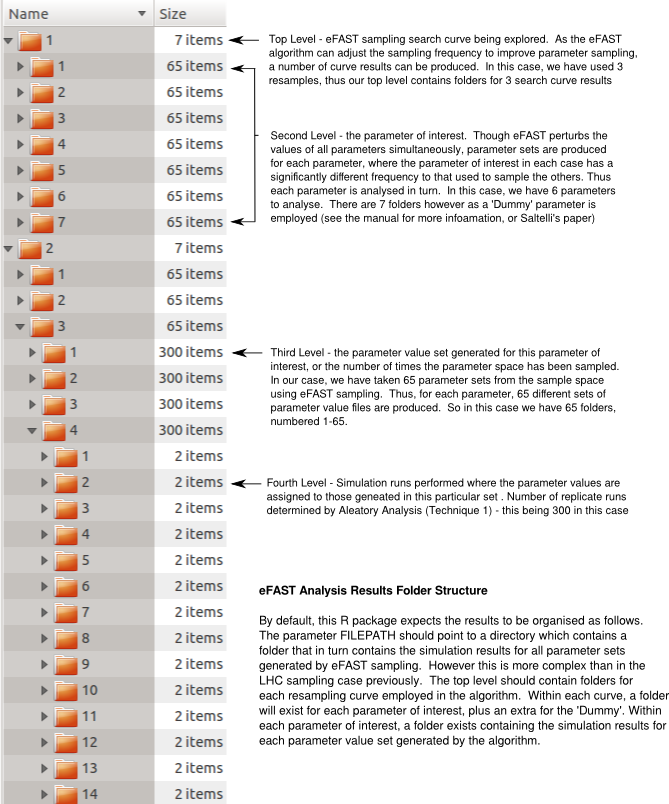
\includegraphics[width=\textwidth]{eFAST_Folder_Struc.png}\\ \noindent
    \caption{Simulation results folder structure that should exist for use with this tool}
    \label{eFAST_Folders}
    \newpage 
\end{figure}

\item With this data available, open the SpartanV Java interface to \textit{spartan}. Select the seventh method from the choice of analysis methods - "Perform analysis for eFAST Generated Samples", and press Next.

\item Firstly, use the Directory Browser to select the folder where you have extracted the tutorial data. Then, you need to enter details of each parameter for which the value has been perturbed. You can do this in two ways:
\begin{itemize}
\item Press the "Add Parameter" button and add details on each parameter individually. These details will be name, baseline (calibrated) value, minimum value, and maximum value.
\item Press the "Add Parameter Values From File" button. This is much more useful if you have a large number of parameters. In this tutorial, press this button and find the Parameter\_Details.csv file you have downloaded from the website. Once you have selected this, the parameter details box will populate, as shown in Figure \ref{eFAST_Screen2}.
\end{itemize}

\begin{figure}
\centering
    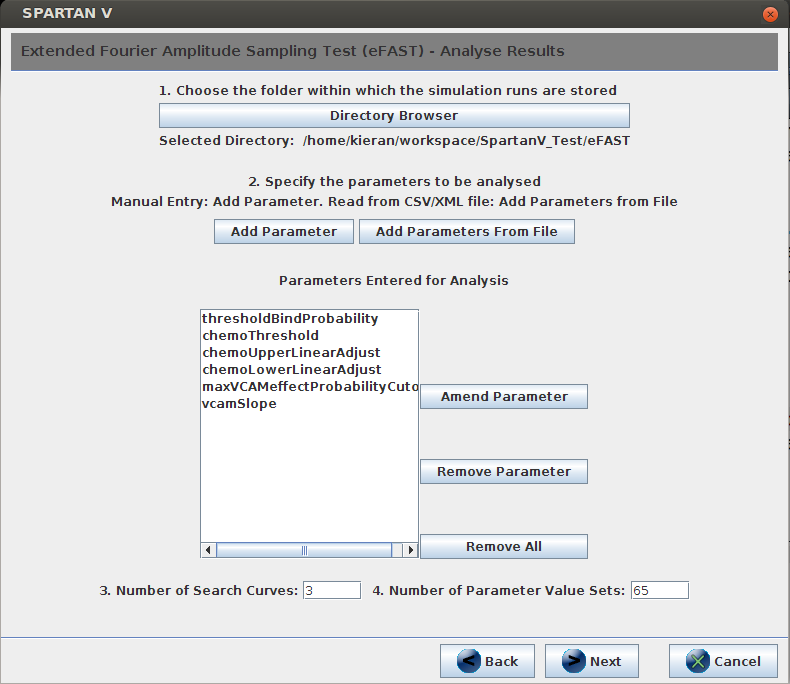
\includegraphics[width=0.8\textwidth]{SpartanV_eFAST2.png}\\ \noindent
    \caption{Specifying parameter details for eFAST analysis}
    \label{eFAST_Screen2}
    \newpage 
\end{figure}

\item In box 3, you specify the number of resample curves that you have employed in sampling, with box 4 the specification of how many values were taken from the parameter search curve. In this example, we employed 3 resample curves and selected 65 values from the parameter space curve. Enter these values into boxes 3 and 4 and press Next.

\item You will now see the screen in Figure \ref{eFAST_Screen3}. This screen requests information about the simulator, in terms of output type (\textit{spartan} can process XML or CSV), result file names, and particular columns where the output responses can be found (if csv). For CSV output, it is good to specify result start and end columns to save R errors on duplicate first column entries, and to save reading in whole CSV files. Finally, the screen requests information on simulation timepoints that are being examined. This is covered later in the tutorial. In this scenario, we assume we are only examining one timepoint, and this the last two input boxes are set to NULL. Complete the input boxes with the data shown in Figure \ref{eFAST_Screen3} and click Next.

\begin{figure}
\centering
    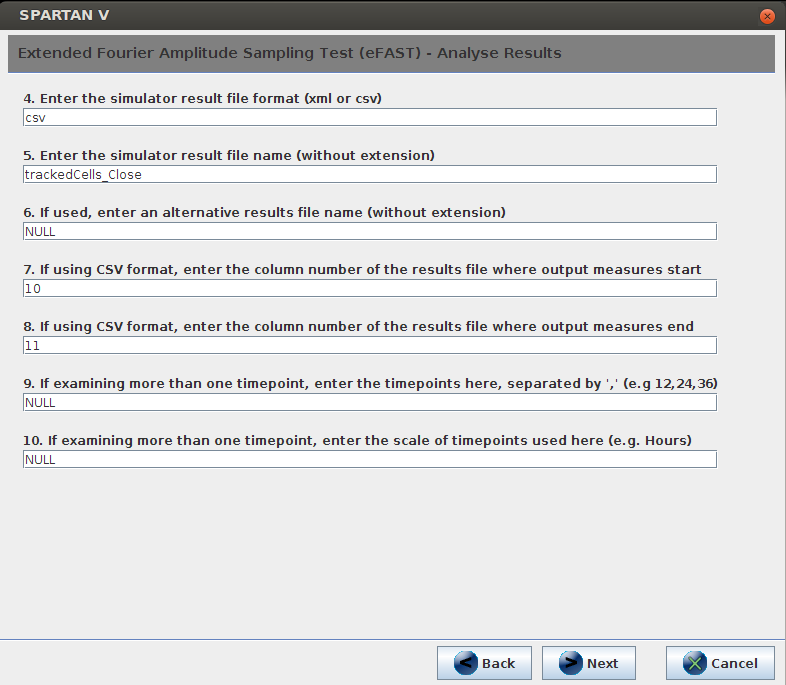
\includegraphics[width=0.8\textwidth]{SpartanV_eFAST3.png}\\ \noindent
    \caption{Specifying simulation specifics for this method of analysis}
    \label{eFAST_Screen3}
    \newpage 
\end{figure}

\item The next screen (as shown in Figure \ref{eFAST_Screen4}) requests information on the simulation output responses that have been examined, the number of replicate runs performed for each parameter value (if this is the case, e.g. for stochastic simulations), and names to assign file names created by the analysis. Complete the remaining data input boxes with the responses in Figure \ref{eFAST_Screen4} and press Next.

\begin{figure}
\centering
    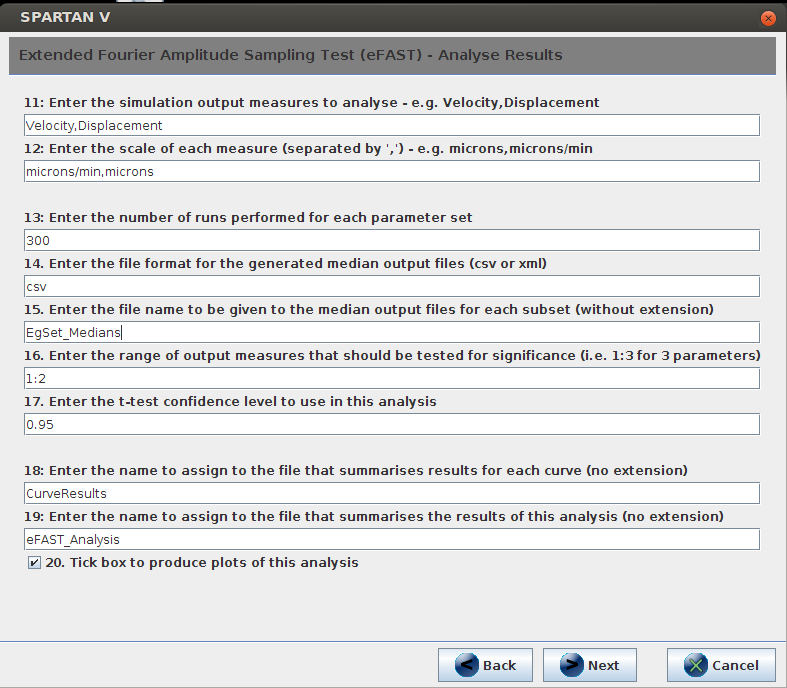
\includegraphics[width=0.8\textwidth]{SpartanV_eFAST4.png}\\ \noindent
    \caption{Specifying simulation specifics for this method of analysis}
    \label{eFAST_Screen4}
    \newpage 
\end{figure}

\item The final screen asks what methods you wish to run in this analysis. Although you would normally run them all, you may want to run some of these separately, or perform them at different times. These are:

\begin{verbatim}
efast_generate_medians_for_all_parameter_subsets(FILEPATH,
	NUMCURVES,PARAMETERS,NUMSAMPLES,NUMRUNSPERSAMPLE,MEASURES,
	RESULTFILEFORMAT,RESULTFILENAME,ALTERNATIVEFILENAME,
	OUTPUTCOLSTART,OUTPUTCOLEND,MEDIANSFILEFORMAT,
	MEDIANSFILENAME)
\end{verbatim}

As stated previously and in other tutorials for this package, a robust representative result is achieved when the simulation is run a number of times for the same parameter conditions. The aim of this method is to examine each parameter value set and produce a file containing the median of each output measure for each simulation run performed under those conditions. In our example case, we know we achieve a representative result if we perform 300 runs of the simulation under the same criteria. The aim therefore is to produce a file which contains the medians of each of our simulation output measures, of each of the 300 runs. We can then use this distribution in comparison with that produced by another parameter value set.
\\
In this case, we examine each resampling curve in turn, and each parameter in turn. Each parameter then has 65 sets of value sets generated in sampling, with each containing 300 simulation runs. When this method is invoked, we will produce a set of medians for each of these 65 value sets, for each parameter. These will be stored in the third level of the folder structure, under the filename specified in the R parameter MEDIANSFILENAME, with file format specified by MEDIANSFILEFORMAT\\

\begin{verbatim}
efast_get_overall_medians(FILEPATH,NUMCURVES,PARAMETERS,
	NUMSAMPLES,MEASURES,MEDIANSFILEFORMAT,MEDIANSFILENAME,
	CURVERESULTSFILENAME)
\end{verbatim}

This method produces a summary of the results for a particular resampling curve. This shows, for each parameter of interest, the median of each simulation output measure for each of the 65 parameter value sets generated.\\
\\
Here's an example. We examine resampling curve 1, and firstly examine parameter 1 (thresholdBindProbability in this case). For this parameter of interest, 65 different parameter value sets were generated from the frequency curves, thus we have 65 different sets of simulation results. The previous method produced a summary showing the median of each output measure for each run. Now, this method calculates the median of these medians, for each output measure, and stores these in the summary. Thus, for each parameter of interest, the medians of each of the 65 sets of results are stored. The next parameter is then examined, until all have been analysed. This produces a snapshot showing the median simulation output for all parameter value sets generated for the first resample curve. These are stored within the second level of the folder structure, with filename as specified by the R variable CURVERESULTSFILENAME.

\begin{verbatim}
efast_run_Analysis(FILEPATH,MEASURES,PARAMETERS,NUMCURVES,
	NUMSAMPLES,OUTPUTMEASURES_TO_TTEST,TTEST_CONF_INT,
	GRAPH_FLAG,CURVERESULTSFILENAME,EFASTRESULTFILENAME,
	TIMEPOINTS,TIMEPOINTSCALE)
\end{verbatim}

Now that these summary files have been produced, we can use the eFAST analysis algorithm in our attempts to partition the output variance between input parameters.  This method creates the file eFAST\_Analysis.csv in the top level of the folder structure (in this case). This contains a number of statistics, for each output measure. The important values are:
\begin{enumerate}[(i)]
\item The Si measure.  Si is the first-order sensitivity index (where i is the parameter).  Calculated as the simulation variance for that parameter over the unique sampling frequency it was assigned, it represents the fraction of model output variance that is explained by an input variation of a given parameter.
\item The STi measure. STi is the total-order sensitivity index (again i is the parameter).  This statistic again indicates the fraction of model output variance, but this time includes any higher-order, non-linear effects between the parameter of interest and its complementary parameters.
\item The SCi measure. SCi is the variance caused by the parameter of interests complementary set (or, all other parameters bar that of interest).
\item Error values.  As the analysis has been done for a number of sample curves, it is possible to calculate other statistical measures such as the standard error. This is useful for plotting the results graphically.
\end{enumerate}

For ease of representation, the method also produces a graph showing this data for each measure.  These will have been saved in the top level directory.

In normal cases, you would now run all of these methods for a simulation such as that in our case study. However, unlike the tutorials on Technique 1 and 2, actual simulation results have not been included in the download due to the excessive file such from such a large number of simulations runs. Instead, the data included is the output of the first method once run. Have a look at one of the files to ensure you understand the format, but we are not going to run this method, else you will get an error in this case. Instead, untick the checkbox for the first method. Your screen should look similar to that in Figure \ref{eFAST_Screen5}. Press Next.

\begin{figure}
\centering
    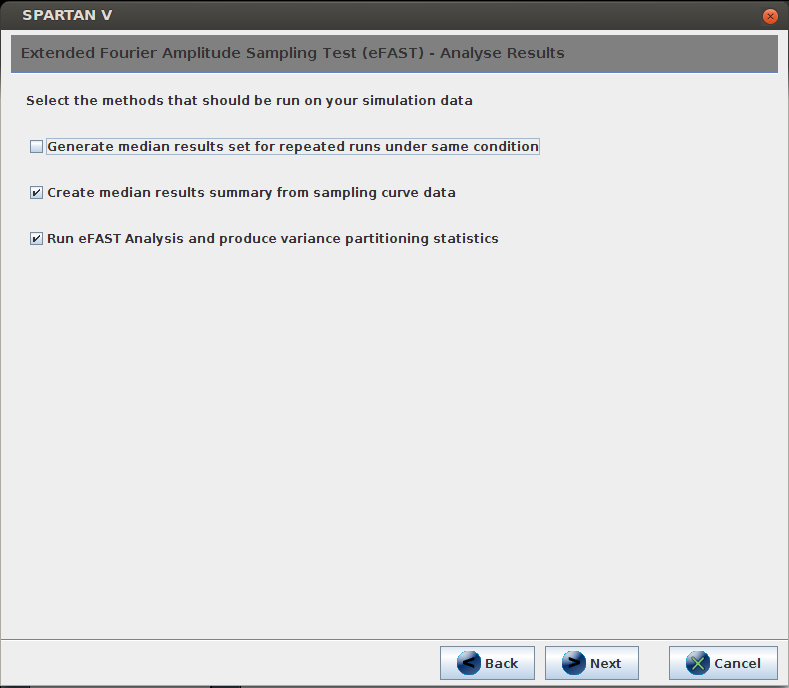
\includegraphics[width=0.8\textwidth]{SpartanV_eFAST5.png}\\ \noindent
    \caption{Selection of methods to run in this analysis. In this case untick the first}
    \label{eFAST_Screen5}
    \newpage 
\end{figure}

\item On the final screen, press the "Run eFAST Analysis" button to start the analysis. The analysis will now run, with updates provided in the console.

Have a look at the output graphs in the top level of the tutorial data folder. You will see that the parameters of interest, and the dummy parameter, are on the x axis. A parameters Si and STi value are deemed significant when a comparison is drawn with the Si and STi of the dummy parameter. In other statistical tests a comparison is made with zero, but that is not possible for eFAST (see Marino paper). So instead the dummy is used. This has no influence on simulation results, but will still be assigned an Si and STi value by the algorithm. Any parameters of interest which have an STi that is less than or equal to the dummy parameter is considered not significantly different from zero.  Comparisons between each parameter of interest and that of the dummy parameter are made using a two-sample t-test. This leads to the calculation of a p-value for the sensitivity indexes, which can also be seen in the summary spreadsheet.  Thus in our example, there are four measures which are significant in terms of affecting a cells velocity (thresholdBindProbability, chemoThreshold, chemoLowerLinearAdjust, maxVCAMeffectProbabilityCutoff).


\end{enumerate}
\newpage 
\begin{figure}[h!]
\centering
    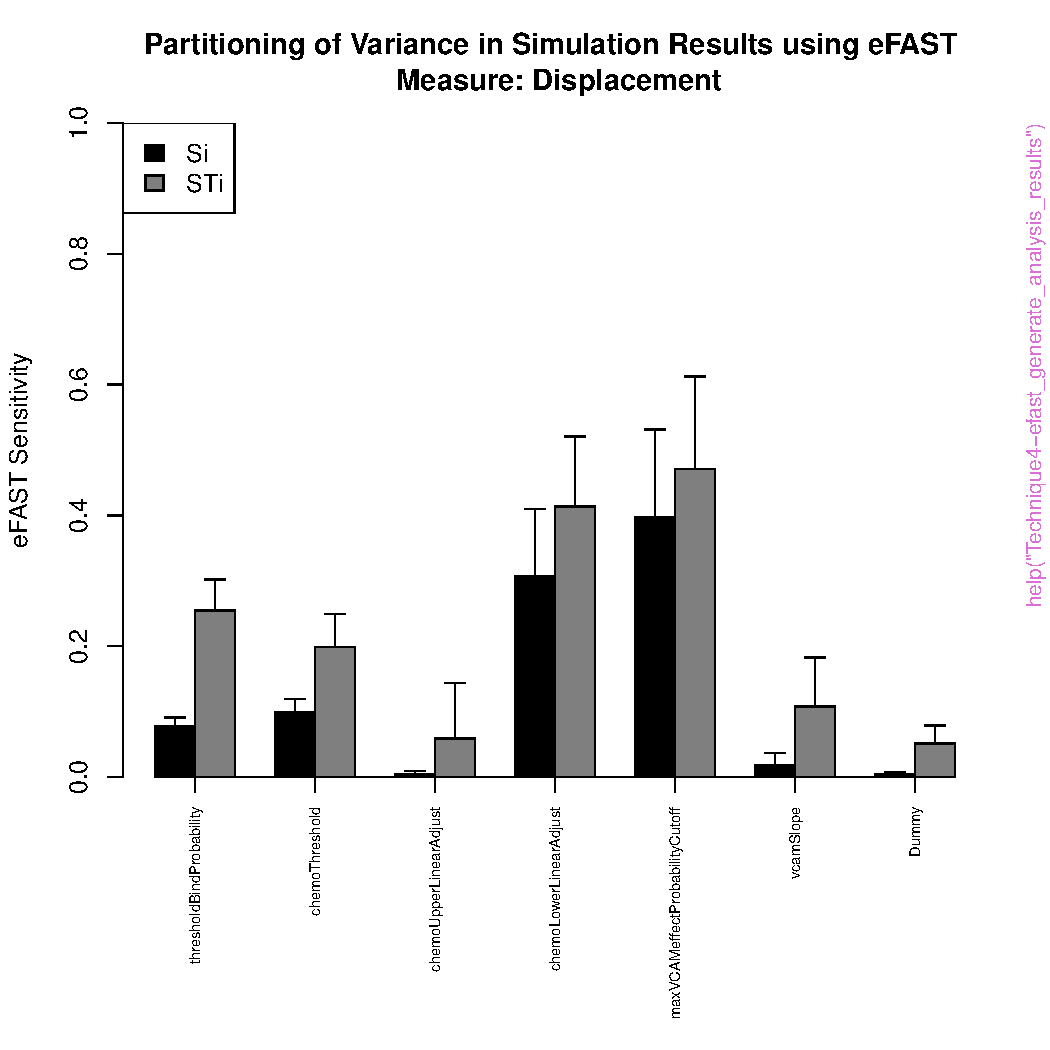
\includegraphics[width=0.65\textwidth]{eFAST_Displacement.pdf}\\ \noindent
    \caption{Graph showing the partitioning of simulation output variance between the input parameters, for the cell displacement measure. Si - Variance accounted for by that parameter; STi - Variance accounted for by its complement set}
    \label{eFAST_Results1}
    \end{figure}

\begin{figure}[h!]
\centering
    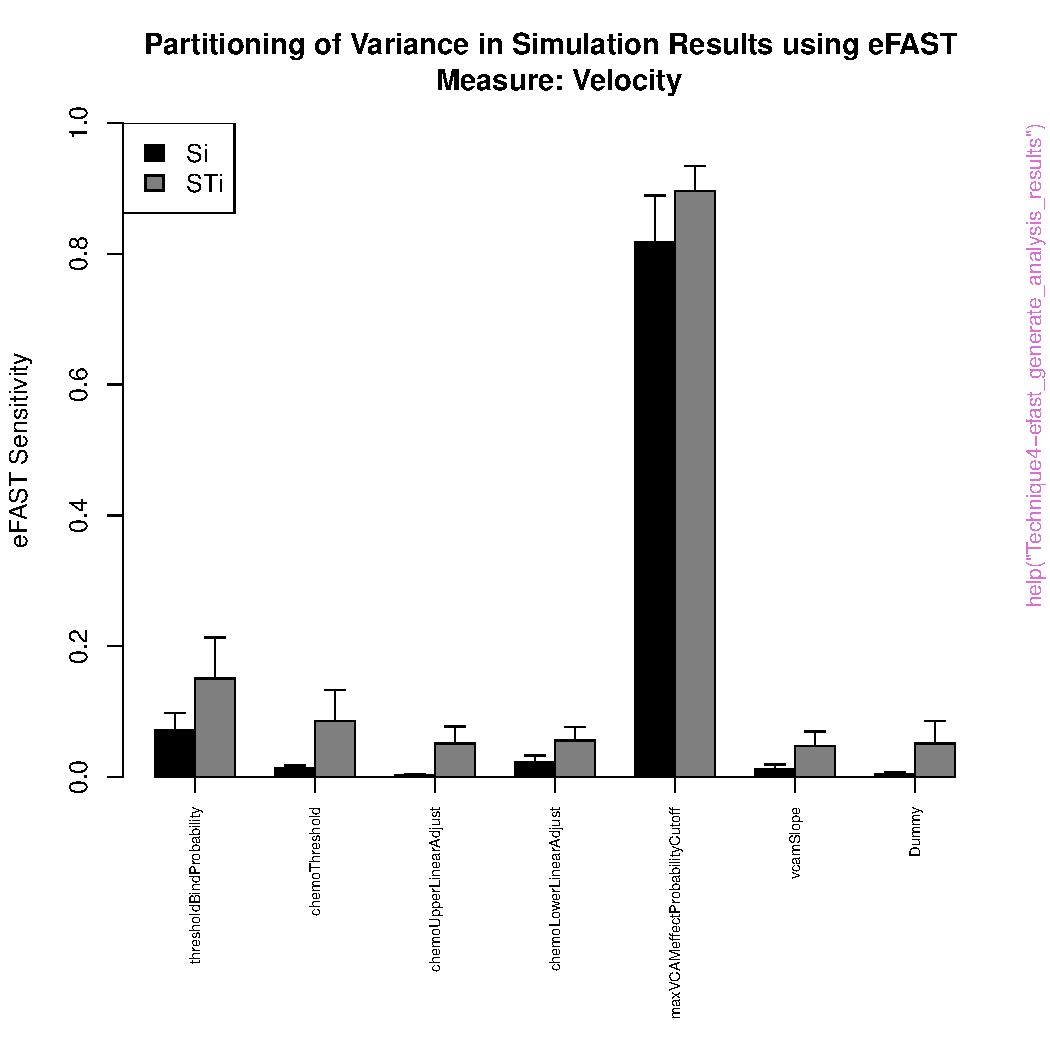
\includegraphics[width=0.65\textwidth]{eFAST_Velocity.pdf}\\ \noindent
    \caption{Graph showing the partitioning of simulation output variance between the input parameters, for the cell velocity measure. Si - Variance accounted for by that parameter; STi - Variance accounted for by its complement set}
    \label{eFAST_Results2}
\end{figure}


\section{Running eFAST Technique for Multiple Timepoints}
\noindent The package also has the capability to perform the above analysis for simulation results taken at different timepoints. This may give an indication of when trends tend to emerge, or certain parameters become influential. Again, we will examine this with an example, yet there is not much to change from the example seen previously\\
\\
In this case study, we have captured the cell behaviour measures at multiple timepoints in the simulation, specifically 12, 36, 48,and 60 hours.  Thus we have the output files trackedCells\_Close\_12.csv, trackedCells\_Close\_36.csv etc. To use this method over multiple timepoints, you should have (a) the same folder structure as in the previous example, and (b) an output file for each timepoint, with the timepoint appended to the filename after an underscore. It is worth writing a script to put your output in this format before looking at this method.\\
\\
We explain how this works through an example, which adapts what we did previously.
\\
Launch the SpartanV interface, and complete Steps 1-5 in the same way as that above. Now, on the second data input screen, enter 12,36,48,60 into box 9 (Timepoints) and type Hours into box 10 (timepoint scale), as seen in Figure \ref{eFAST_Screen6}. This tells the analysis that you want to examine simulation responses at four different time-points, with the latter used for graphing results in the final part of the method. Press Next and complete the other data entry screens in the same way. Run the analysis, and statistics will be produced for all four timepoints. 

\begin{figure}
\centering
    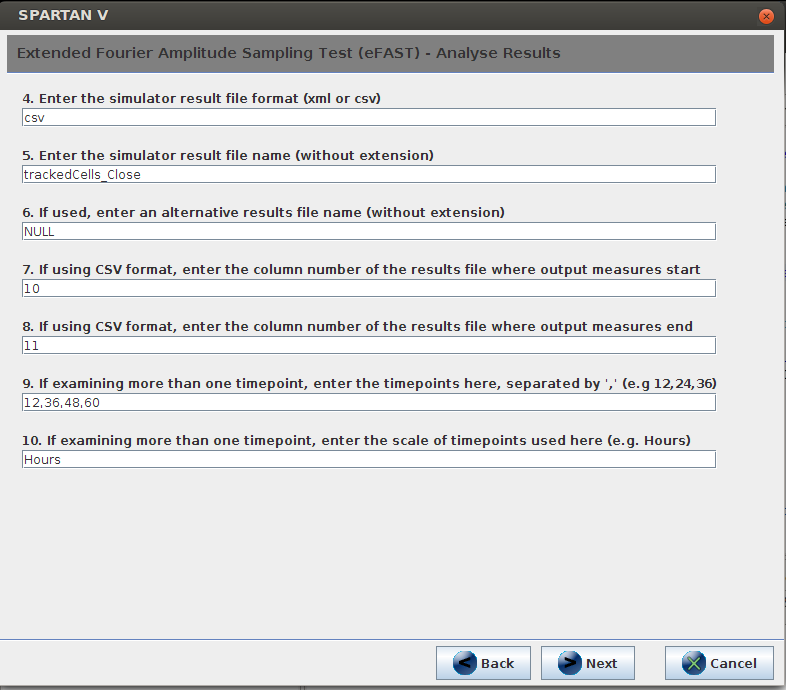
\includegraphics[width=0.8\textwidth]{SpartanV_eFAST6.png}\\ \noindent
    \caption{Adding additional time-points to observe effect of parameter perturbation over time}
    \label{eFAST_Screen6}
    \newpage 
\end{figure} 

\section{Further Reading}
\noindent
The following references may be useful in understanding this technique in more detail:
\begin{itemize}
\item Read, M., Andrews, P.S., Timmis, J. \& Kumar, V. (2012) Techniques for Grounding Agent-Based Simulations in the Real Domain : a case study in Experimental Autoimmune Encephalomyelitis. Mathematical and Computer Modelling of Dynamical Systems, 18(1):67-86.
\item Marino, S., Hogue, I.B., Ray, C.J. \& Kirschner, D.E. (2008) A methodology for performing global uncertainty and sensitivity analysis in systems biology. Journal of theoretical biology, 254 (1), p.pp.178-96.
\item Saltelli, A., Chan, K. \& Scott, E.M. (2000) Sensitivity Analysis, Wiley series in probability and statistics Wiley.
\item The spartan Manual, spartan-Manual.pdf, within the spartan package describes in more detail each method within the package
\end{itemize}


\end{document}